\chapter{Trajectory Planning}
\label{ch:trajectory}

\section{Joint-space and Cartesian-space paths}
A path specifies the geometric states to visit; a time law specifies how fast
to traverse them. Joint-space planning directly interpolates the six
coordinates $q_i$. Cartesian planning specifies a straight-line tool-position
segment and a fixed tool orientation, then solves IK at each sampled point.
The project uses both: the initial approach uses a joint-space quintic
segment, while descent/lift/transfer/lower/retreat use Cartesian segments.

The Cartesian tool orientation is fixed to
\begin{equation}
 R_{down}=\mathrm{diag}(1,-1,-1),\qquad \det(R_{down})=+1,
\end{equation}
which is a 180-degree rotation about base/tool x: tool $+x$ stays $+X$, while
tool $+y$ and $+z$ reverse. The matrix is a proper rotation and points the
grasp direction downward under this tool convention.

\section{Quintic time scaling}
For normalized time $u=t/T\in[0,1]$, the implemented blend is
\begin{equation}
 s(u)=10u^3-15u^4+6u^5.
 \label{eq:quintic}
\end{equation}
Its derivatives are
\begin{align}
 s'(u)&=30u^2-60u^3+30u^4,\\
 s''(u)&=60u-180u^2+120u^3.
\end{align}
At $u=0$ and $u=1$, $s$ reaches its endpoint values while $s'$ and $s''$ are
zero. This gives a rest-to-rest scalar interpolation with zero endpoint
velocity and acceleration for a linearly parameterized coordinate. The
dimensionless derivatives are scaled by $1/T$ and $1/T^2$ for physical
velocity and acceleration.

\begin{figure}[htbp]
\centering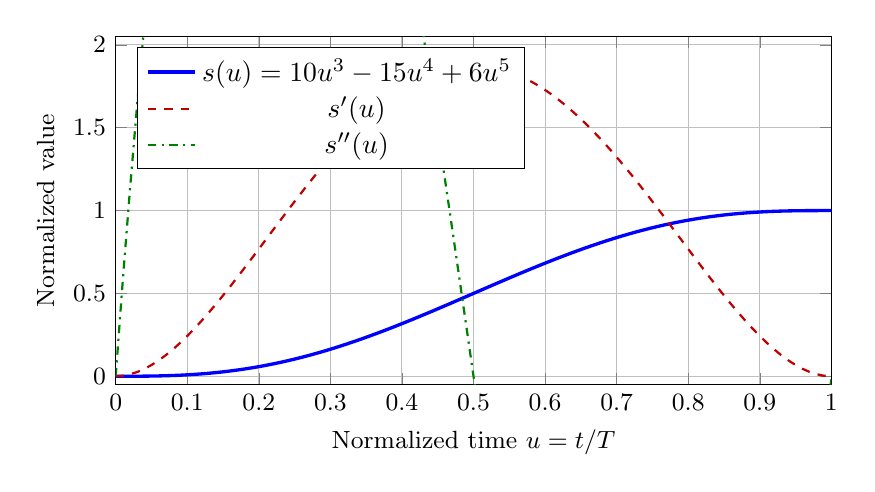
\begin{tikzpicture}
\begin{axis}[
  width=.88\textwidth,height=6cm,
  xlabel={Normalized time $u=t/T$},ylabel={Normalized value},
  xmin=0,xmax=1,ymin=-.05,ymax=2.05,
  grid=both,legend pos=north west,
  tick label style={font=\small},label style={font=\small},
  domain=0:1,samples=100
]
\addplot[blue,very thick] {10*x^3-15*x^4+6*x^5};
\addlegendentry{$s(u)=10u^3-15u^4+6u^5$}
\addplot[red!75!black,thick,dashed] {30*x^2-60*x^3+30*x^4};
\addlegendentry{$s'(u)$}
\addplot[green!50!black,thick,dashdotted] {60*x-180*x^2+120*x^3};
\addlegendentry{$s''(u)$}
\end{axis}
\end{tikzpicture}

\caption{Position blend and its derivatives for the quintic scalar time law.
This is the intended analytical profile, not a measured joint trace.}
\label{fig:quintic}
\end{figure}

For a joint-space segment, the code applies this blend directly:
\begin{equation}
 q(t)=q_0+s(t/T)(q_f-q_0),\quad
 \dot q(t)=\frac{s'(t/T)}{T}(q_f-q_0).
 \label{eq:joint-quintic}
\end{equation}
It samples at approximately \SI{50}{ms} intervals. The base duration defaults
to 8 s for the approach, then time-stretches if a sampled speed exceeds the
allowed joint speed cap.

\section{Cartesian segment construction}
For a Cartesian segment from $p_0$ to $p_f$, the implementation evaluates
\begin{equation}
 p(u)=p_0+s(u)(p_f-p_0),\qquad R(u)=R_{down}.
\end{equation}
It generates samples with nominal interval no greater than \SI{50}{ms}, solves
IK sequentially using the preceding $q$ as the next seed, and stores each
joint solution. The segment refuses to start unless its current tool
orientation is within $10^{-4}$ rad of the downward target. It refuses a
joint branch with adjacent sampled joint displacement above 0.15 rad.

Because the mapping $p\mapsto q$ is nonlinear, the resulting $q_i(t)$ values
do not each follow the scalar quintic equation exactly. The implementation
estimates joint velocity using \code{numpy.gradient} over sampled IK points,
then forces the first and last velocity vectors to zero. Unlike the joint
segment, it does not compute the analytic second derivative of the IK path.
The theoretical zero endpoint Cartesian acceleration should therefore not be
reported as a measured joint-acceleration guarantee.

\section{Velocity cap and duration stretching}
The allowed speed per joint is
\begin{equation}
 v_{cap,i}=\min(v_{URDF,i},0.5\si{rad/s}).
\end{equation}
For sampled joint speed estimates, the time scale is
\begin{equation}
 \lambda=\max\left(1,\max_{k,i}\frac{|\dot q_{k,i}|}{v_{cap,i}}\right).
 \label{eq:time-stretch}
\end{equation}
The code multiplies all timestamps by $\lambda$ and divides the sampled
velocities by $\lambda$. It samples and checks velocity; it does not impose a
measured acceleration or jerk limit. This is reference-trajectory scaling,
not feedback torque/velocity control. The Gazebo controller's position
command interface tracks the supplied trajectory.

\section{Scene-specific waypoint schedule}
The far route avoids a diagonal sweep through the base. It first descends to
the pickup (5 s), lifts to $z=0.10$ m (5 s), moves inward and gains height
through $(0.45,-0.45,0.40)$ m (7 s), transfers above Box A at $z=0.40$ m (6 s),
lowers to $z=0.226$ m (4 s), and retreats to the overhead target (4 s). The
initial approach to the above-pickup posture has nominal duration 8 s. Near
pickup instead lifts directly to $z=0.40$ m before transfer. These durations
are nominal; time scaling can extend them. They are hand-designed for this
scene and are not generated by collision search.

\section{Controller sampling and what is actually smooth}
The planned arrays are serialized into trajectory points with position,
velocity, and relative time. The arm controller exposes a position command
interface and position/velocity state interfaces. The quintic curve is smooth
within each generated segment at the scalar level, but the project does not
record per-joint traces, compute inter-segment acceleration discontinuity, or
validate jerk. The offline test resamples joint trajectories with a cubic
Hermite spline and checks sampled bounds, speed, endpoint, and orientation; it
does not prove Gazebo's exact interpolation or physical drive behavior.
